%!TEX root = ../document.tex
\chapter{实验结果与分析}

\section{数据集介绍}

为了比较上文提出的两个算法模型,分别从推荐结果的准确性、和算法训练与结果查询返回效率两个方面分别进行了两组实验。%
因此需要设计两组实验分别从算法推荐准确性和性能两个方面进行验证。本文评估了上述两个算法在两个来自真实%
应用的数据集上,这些数据集都包涵用户与物品产生交互的时间戳:

\textbf{MovieLens}:MovieLens\footnote{\url{https://grouplens.org/datasets/movielens/}}是%
用来对推荐模型进行评估的最流行的基准数据集,它是由GroupLens研究组织从MovieLens网站收集的关于用户%
对电影评分的数据集,其中主要的评分文件以“用户ID | 电影ID | 评分 | 时间戳”为一行的格式%
保存了某个用户在某时刻对某个电影做出的评分标准,按照数据量的大小不同,本文选用的MovieLens数据集是%
Movielens-1M。

\textbf{Yoochoose}:Yoochoose\footnote{\url{http://2015.recsyschallenge.com}}数据集是%
2015年推荐系统顶级会议RecSys举办的挑战赛RecSys Challenge 2015上公开使用的目标数据集。%
Yoochoose包含了一个在线电子商务网站在6个月时间内用户所有的点击会话流和购买会话流。这里本文只使用了%
点击会话流数据集“yoochoose-clicks.dat”,其中每一行包含了一个点击交互行为,总共有33003944行,%
并抽取了其中的前100万行进行建模实验。%
\begin{table}[]
  \centering
  \caption{序列数据集对比}
  \label{tab:datatable}
    \begin{tabular}{@{}lllllll@{}}
    \toprule
    数据集名称    & 物品数目 & 序列数目 & 交互行为数目 & 平均序列长度  \\ \midrule
    MovieLens-1M & 3706     & 6040 & 1000000 & 165.56 \\
    Yoochoose    & 20843 & 254619 & 1000000 & 3.93 \\ \bottomrule
    \end{tabular}
\end{table}
对于每一种数据集,在特征工程处理部分,需要将其处理成按时间排列的序列,因此需要将交互行为按照时间戳进行预排序,%
将排序好的交互行为按照其所属用户或会话流分组构成序列集合。图\ref{fig:feature_engine}以Movielens-1M数据集%
为例,特征工程前后数据结构示意图,Yoochoose数据集特征工程与此相同。
不同的算法使用的数据集划分策略不同,下文针对每种算法将详细描述数据集划分策略。具体实验数据明细如表格\ref{tab:datatable}所示。
\begin{figure}[!htb]
   \begin{minipage}{0.48\textwidth}
     \centering
     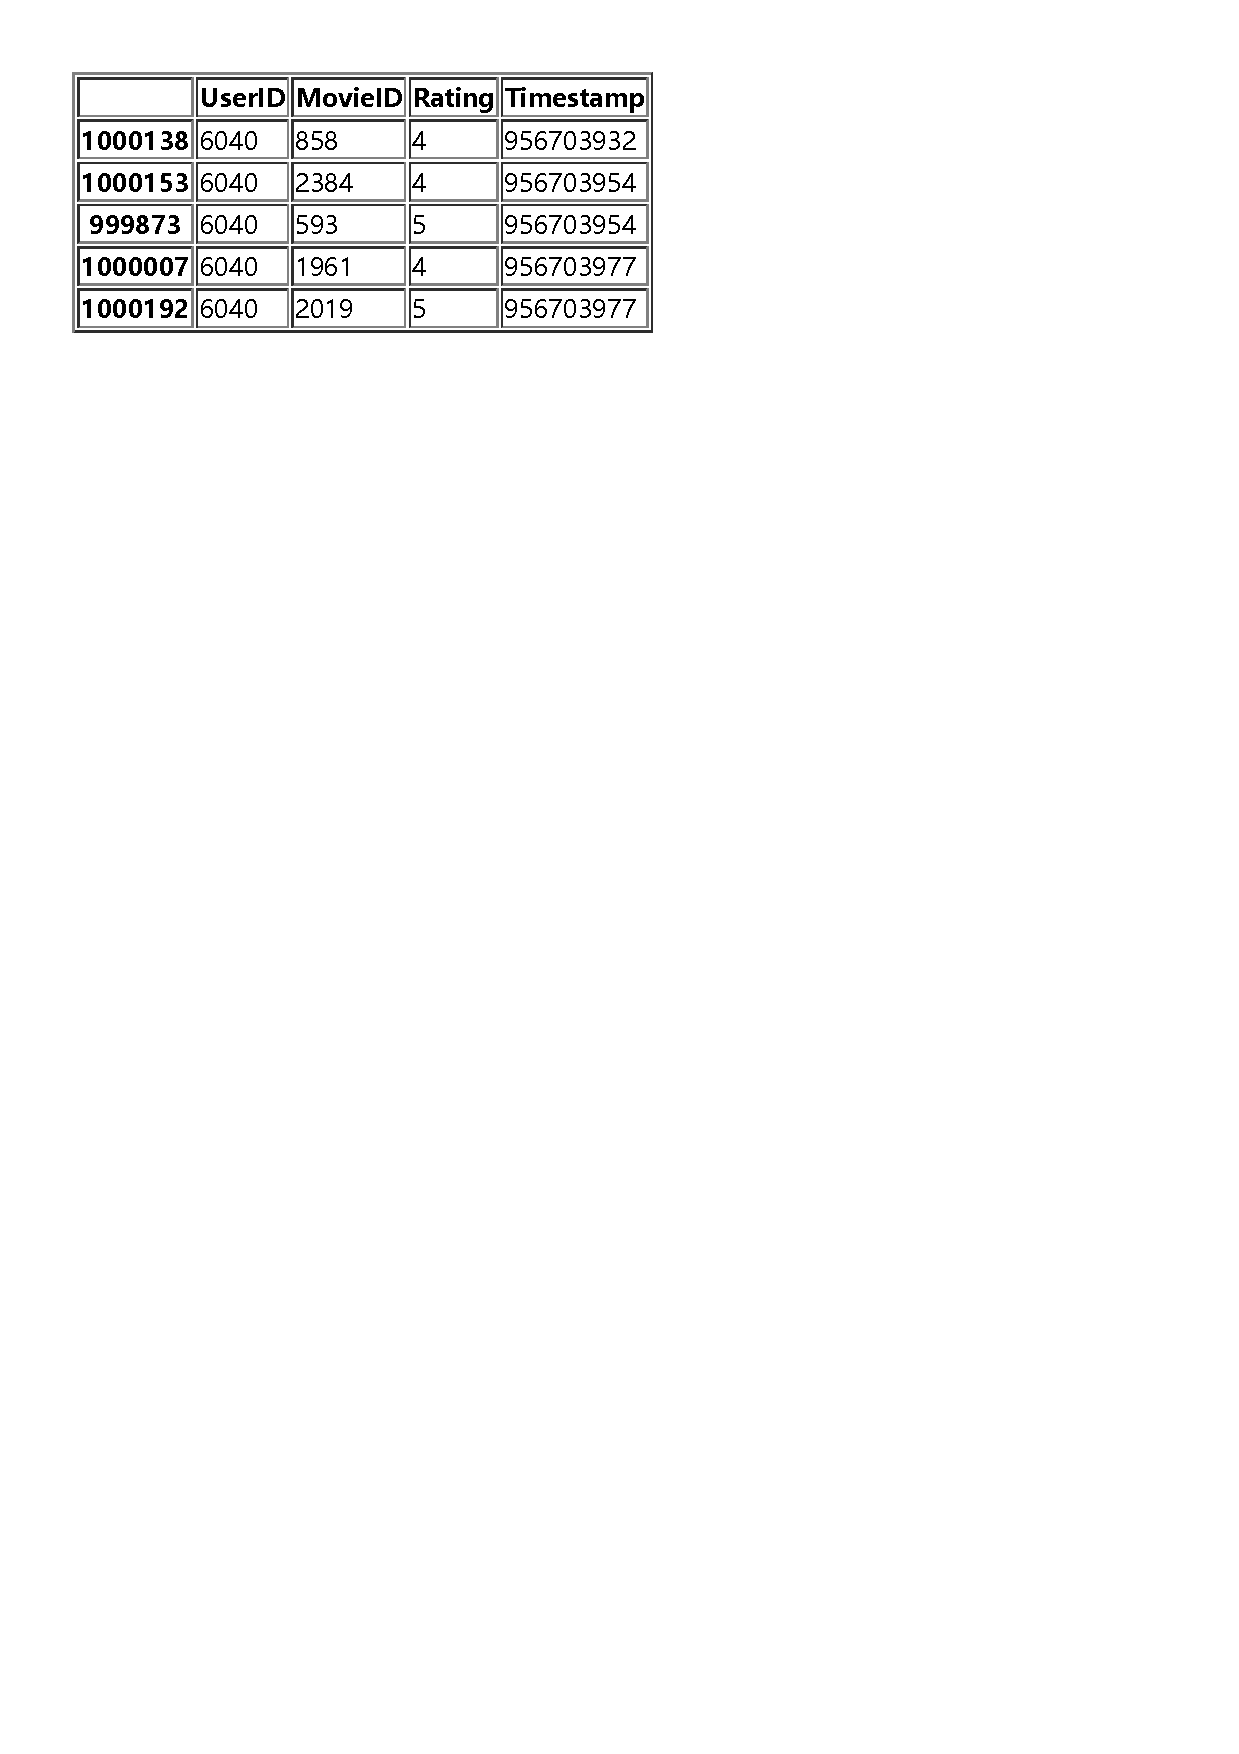
\includegraphics[height=3cm]{MLtable.pdf} % ,width=\linewidth
     \caption{原始数据}
     % \label{Fig:MLtable}
   \end{minipage}\hfill
   \begin {minipage}{0.48\textwidth}
     \centering
     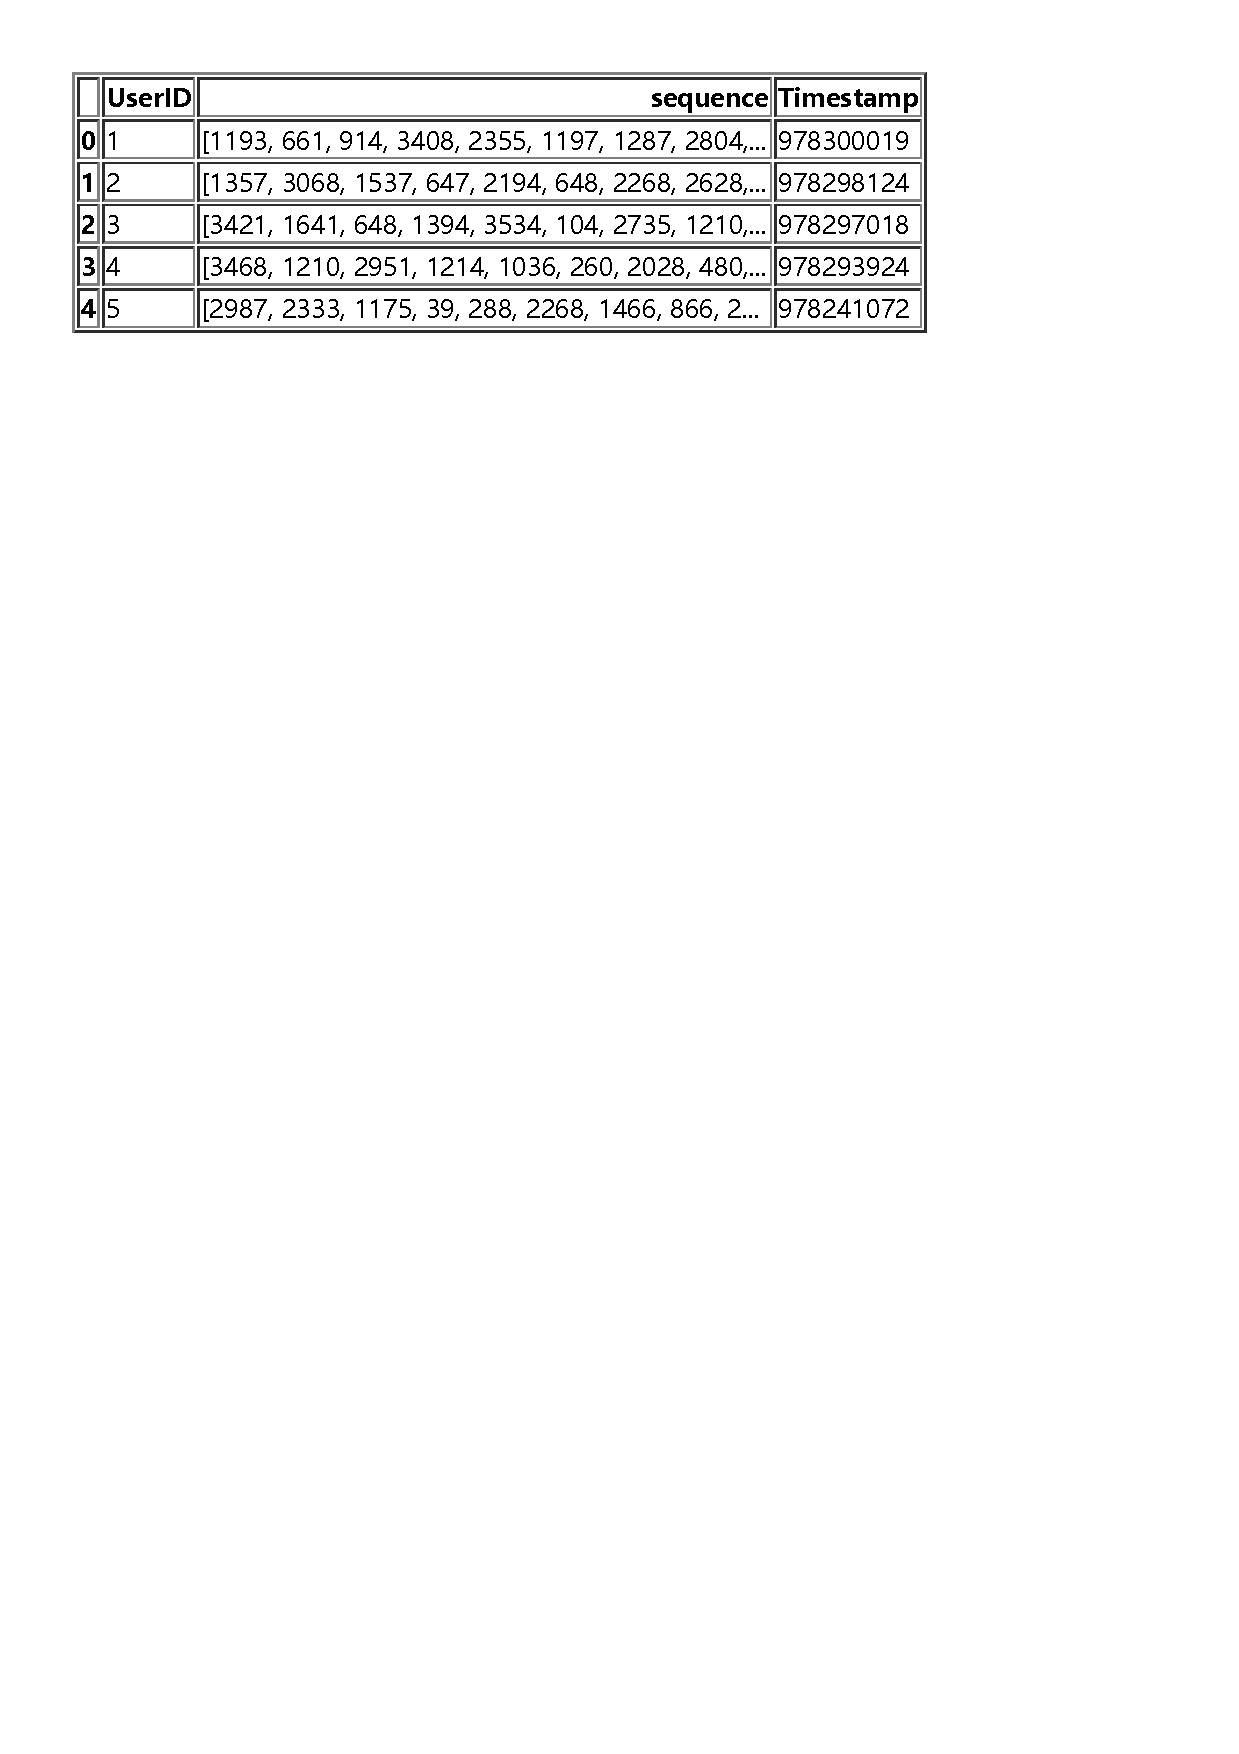
\includegraphics[height=3cm]{MLsequence.pdf} % ,width=\linewidth
     \caption{特征工程处理后数据}
     % \label{Fig:MLsequence}
   \end{minipage}
   \caption{以Movielens-1M数据集为例,将原始交互数据按时间戳排序后分组构成行为序列}
   \label{fig:feature_engine}
\end{figure}


\section{评价指标}
作为一个推荐模型,模型会对查询目标给出点击可能性最高的N个物品,对于本文提出的序列推荐形式,%
模型的输入是$t$时刻及其以前的用户点击物品序列,需要的模型输出目标是$t+1$时刻用户可能点击%
的物品,以$\hat{I}_{u}^{t+1}$表示,所以本文采用了$Precision@N$, $Recall@N$指标来评估%
本文的模型,其计算形式如下:
\begin{equation}
Precision@N=\frac{\sum_{u}|\hat{I}_{u}^{t+1}\cap I_{u}^{t+1} |}{\left | \mathbb{U} \right |*N}
\end{equation}
\begin{equation}
Recall@N=\frac{\sum_{u}|\hat{I}_{u}^{t+1}\cap I_{u}^{t+1} |}{\left |\sum_{u}|I_{u}^{t+1}| \right |}
\end{equation}
由于$Precision@N$和$Recall@N$值可以通过阈值调整来相互权衡,为了得到一个更加容易量化评估%
的指标,本文引入了$F1@N$指标,如果$F1@N$分数越大,可以认为模型的效果更好。而当一次为%
用户推荐多个结果时,推荐结果在屏幕上展示的位置也会影响物品被点击的概率,越靠前的物品越可能被点击,%
约强相关的推荐物品应该出现在结果列表的越前面,而引入$NDCG@N$\upcite{NIPS2009_3758}指标的原因就是为了感知这种%
位置的影响,让点击率越高的物品位置越靠前,$NDCG@N$%
值越接近1,得到的相关推荐结果中前N个物品的排序越准确,所以$F1@N$和$NDCG@N$的计算形式如下:
\begin{equation}
F1@N=\frac{2\times Precision@N\times Recall@N}{Precision@N+Recall@N}
\end{equation}
\begin{equation}
  \begin{aligned}
  DCG@N &= \sum_{i=1}^{N} \frac{2^{rel_{i}}-1}{\log _{2}(i+1)} \\
  IDCG@N &= \sum_{i=1}^{|REL|} \frac{2^{rel_{i}}-1}{\log _{2}(i+1)} \\
  NDCG@N &= \frac{DCG@N}{IDCG@N}
  \label{E21}
  \end{aligned}
\end{equation}
当推荐的物品是用户点击的内容时$DCG@N$中$rel$取值为1,否则$rel$取值为0。而由于每条样本仅有一条为相关,其余均为不相关,所以 $IDCG@N$ 对于每条样本都是一样的,即$\frac{1}{\log 2}$。

\section{实验环境}
本文面向序列感知推荐算法设计了基于循环结构的BiLSTM4Rec和基于自注意力机制的Transformer4Rec模型,其模型的软硬件环境以及工具如表\ref{tab:set}所示。
\begin{table}[H]
\centering
\caption{实验软硬件环境配置表}
\label{tab:set}
  \begin{tabular}{@{}ll@{}}
  \toprule
  实验环境 & 环境配置                                  \\ \midrule
  CPU  & Intel(R) Xeon(R) CPU E5-2650 v3 @ 2.30GHz *2 \\
  GPU  & Tesla K80 *4                                 \\
  内存   & 64126MB                                      \\
  OS   & CentOS Linux 7 (Core)                        \\
  编程语言 & Python 3.6.8                                 \\
  开发工具 & TensorFlow-GPU 1.12.0                        \\ \bottomrule
  \end{tabular}
\end{table}

\section{基于双向LSTM的序列感知算法实验过程}

本节将通过实验来验证第三章中提出的基于双向LSTM的序列感知算法BiLSTM4Rec的有效性,主要介绍针对该实验的数据集处理策略、实验主要研究的问题、影响结果的主要因素。
基于双向LSTM的序列感知算法的特征工程部分,首先将每个交互样本按照时间戳从先到后排列,然后根据交互样本所属用户聚类构成行为序列,在序列感知推荐算法当中不需要用户的评分数据因此可以去除。对于行为序列长度小于5的序列进行了过滤,剩余序列集合前80\%划分为训练集,后20\%划分为测试集。将序列中最后一个交互物品ID作为模型学习的标签,截取序列中最近的$N$个物品作为BiLSTM的输入序列,其中$N\geq 1$,当$N>1$而存在序列的长度不足时,在长度不足序列的前部进行特殊值填充以表示缺失。当时间窗口为1时,意味着我们将序列的最后一个物品作为标签,最近的一个物品作为序列的特征输入模型就行学习。

BiLSTM4Rec模型的实现基于开源深度学习框架Keras,以Tensorflow作为其后端。使用批量梯度下降法Adam作为优化器,并设置初始学习率$\alpha$为0.01,学习率衰减权重因子$\beta$为0.9。其他超参数本实验首先使用常见值作为初始值,为了得到更好的性能,使用网格搜索的形式自动寻找最优参数组合,但这会带来极大的计算量。经过多次尝试,本实验最终选定了以下超参数组合:嵌入层因子$|e|=100$,循环层神经元数目$H=200$,全连接层神经元数目$O=100$,梯度下降批量大小为32。在训练阶段为避免过拟合,当验证数据上经过3个batch损失函数仍没有下降则EarlyStopping。

为了探求基于双向LSTM的序列感知算法需要的序列长度,将超参数固定之后本文也设置了对比实验探求不同序列长度对模型的影响,图\ref{fig:windows}显示了在MovieLens-1M数据集上输入序列长度分别从$1\sim 10$时,训练阶段EarlyStopping时最优的损失函数值。
\begin{figure}[htb]%更改
  \centering
  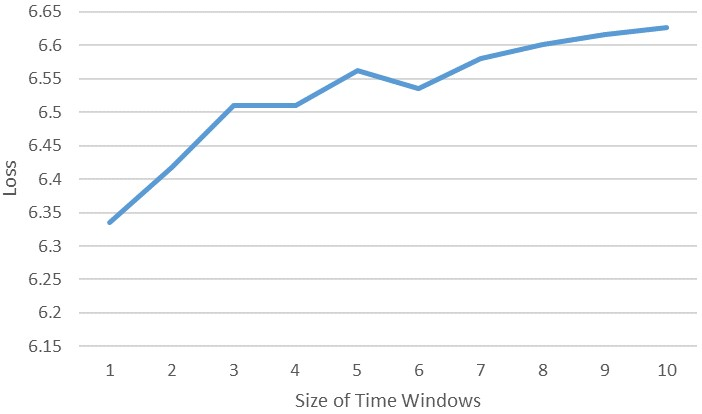
\includegraphics[width=12cm]{Loss_timewindows.jpg}
  \caption{BiLSTM4Rec在MovieLens-1M数据上不同序列长度的最小训练loss}
  \label{fig:windows}
\end{figure}
通过图\ref{fig:windows}中可以看到,在不同的输入序列长度下,BiLSTM的性能有稍微的降低,为了模型的稳定性选取了中位值5作为最终序列长度。
图\ref{fig:BiLSTMloss}显示了固定时间窗口为5及其他超参数的情况下,训练集和测试集上的损失函数下降图。
\begin{figure}[htb]%更改
  \centering
  \includegraphics[width=12cm]{model_loss-eps-converted-to.pdf}
  \caption{BiLSTM4Rec在MovieLens-1M数据上不同序列长度的最小训练loss}
  \label{fig:BiLSTMloss}
\end{figure}

\section{基于自注意力机制的序列感知算法实验过程}
本节将通过实验来验证第四章中提出的基于自注意力机制的序列感知算法Transformer4Rec的有效性。
与基于双向LSTM的序列感知算法的特征工程部分一样,首先将每个交互样本按照时间戳从先到后排列,然后根据交互样本所属用户聚类构成行为序列。
在数据集划分部分,由于基于自注意力机制的序列感知算法包含Encoder-Decoder结构,Decoder对应的输出序列由输入序列往后滑动一个窗口构成,
在数据集划分部分也使用了同样的划分策略,将所有序列截止倒数第三个位置之前部分划分为训练集,截止倒数第二个之前部分划分为验证集,包含最后一个物品的序列作为测试集,超过最大长度$N$部分做截取处理。

图\ref{fig:Slefattentionloss}为学习率分别设置为0.001、0.003、0.01时训练集上的损失函数的下降曲线,从图中可以看到,
Transformer4Rec模型在MovieLens-1M上使用合适的学习率损失函数可以更快收敛,节省训练时间,因此后文实验以学习率0.01为基础进行。
\begin{figure}[htb]%更改
  \centering
  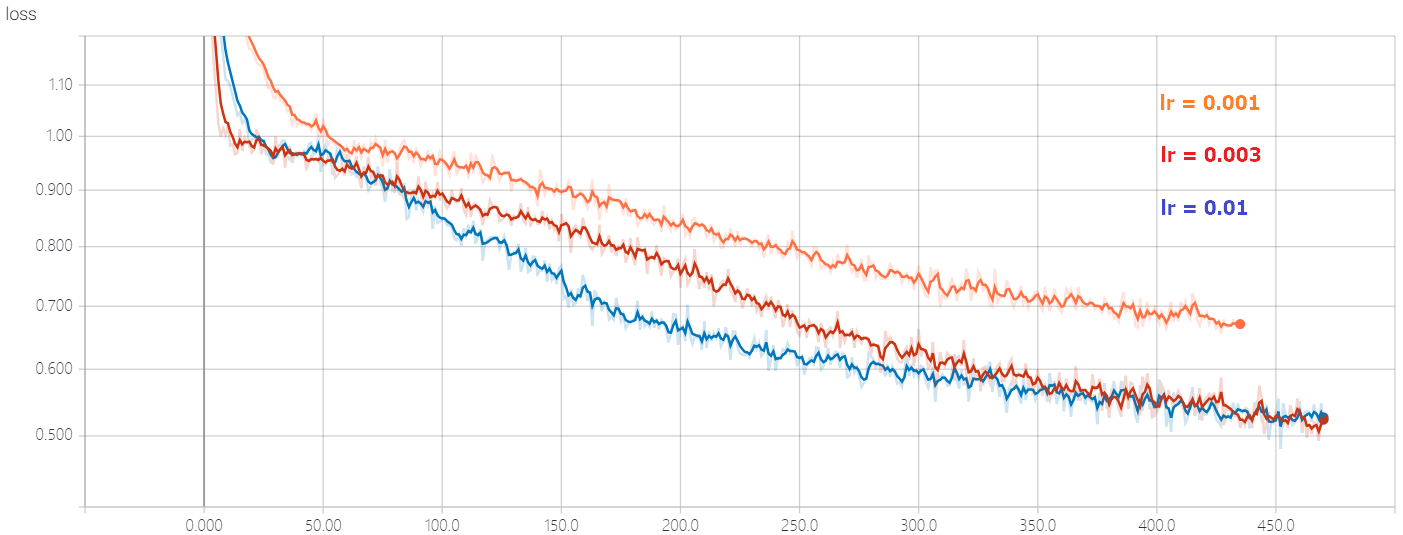
\includegraphics[width=12cm]{2019-03-31-174902.png}
  \caption{Transformer4Rec在MovieLens-1M数据上学习率分别设置为0.001、0.003、0.01时训练集上的损失函数的下降曲线}
  \label{fig:Slefattentionloss}
\end{figure}

模型输入序列的长度也是影响模型性能的关键因素之一,在固定学习率及其他超参数之后本节试验了不同长度序列对模型性能的影响,如图
\ref{fig:maxlenloss}所示,从图中可以看到不同序列长度对模型性能的影响不是非常明显,但越长的序列它的迭代过程越慢,综合考虑
性能与效率的原因,在本节MovieLens-1M数据集上最大序列长度设为150,在Yoochoose数据集上最大长度设为50。
\begin{figure}[htb]%更改
  \centering
  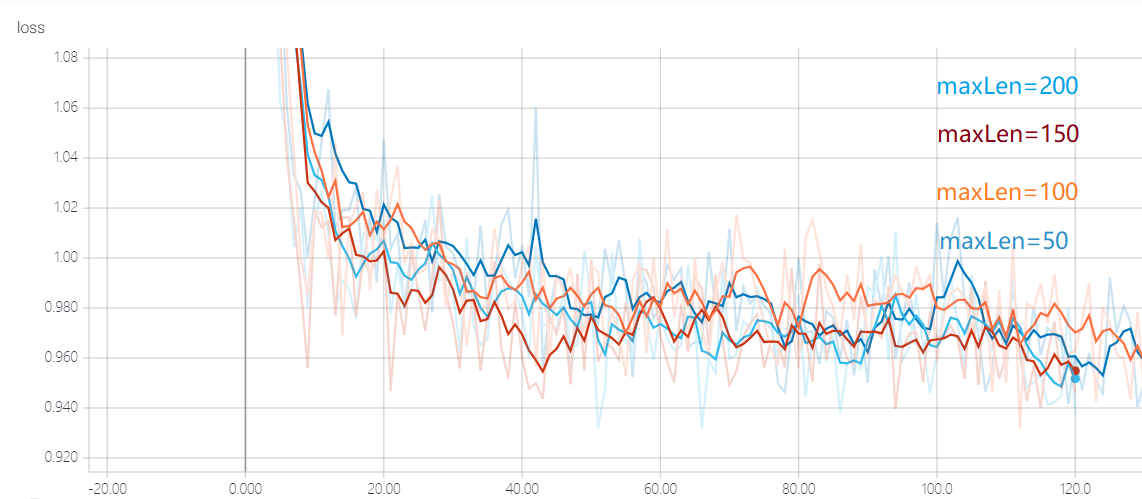
\includegraphics[width=12cm]{2019-03-31-220433.png}
  \caption{Transformer4Rec在MovieLens-1M数据上最大序列长度分别设置为200、150、100、50时训练集上的损失函数的下降曲线}
  \label{fig:maxlenloss}
\end{figure}
其他重要超参数如Dropout比率、Multi-Head Attention中Self-Attention个数、批量大小、迭代次数、隐藏层神经元数目等,经过
自动网格搜索后分别确定为:0.2、2、128、10、50。

% \subsection{实验三}

\section{对比实验}
\subsection{算法测评指标对比}
\textbf{POP}:最流行物品推荐法POP作为本文选择的最简单的基准线,通过统计训练数据中出现次数最多的物品,推荐策略为为用户推荐那些他还没有看过的最热门的物品。

\textbf{GRU4Rec\upcite{DBLP:journals/corr/HidasiKBT15,Hidasi:2018:RNN:3269206.3271761}}:GRU4Rec是序列感知推荐领域最重要的算法之一,2016年Balazs Hidasi等人首次将循环神经网络的方法应用到基于会话的个性化推荐领域,并取得了当时的最好效果,因此本文将其作为\textit{基于循环神经网络的序列感知推荐算法}中的代表,其代码基于Keras\footnote{\url{https://keras.io}}提供的GRU高层API实现。

\textbf{Caser\upcite{Tang:2018:PTS:3159652.3159656}}:2018年Jiaxi Tang等人将序列嵌入矩阵使用CNN提取特征,提出了卷积序列嵌入推荐模型Caser,因此本文将其作为\textit{基于卷积神经网络的序列感知推荐算法}中的代表,其代码实现基于原作者开源的PyTorch实现版本\upcite{paszke2017automatic}。

本文讨论的两个模型与三个对比模型的分别在MovieLens-1M与Yoochoose数据集上的实验结果如表\ref{table:result}所示。

% Please add the following required packages to your document preamble:
% \usepackage{booktabs}
% \usepackage{multirow}
\begin{table}[]
\centering
\caption{各算法评价指标结果}
\label{table:result}
  \begin{tabular}{@{}lllllll@{}}
  \toprule
  数据集名称                     & 测评指标      & POP      & GRU4Rec  & \textbf{BiLSTM4Rec} & Caser & \textbf{Transformer4Rec} \\ \midrule
  \multirow{4}{*}{MovieLens-1M} & Recall@10    & 0.041390 & 0.109286 & 0.125679 & 0.1344 & 0.7055      \\
                                & Precision@10 & 0.004139 & 0.010928 & 0.012567 & 0.0112 & 0.0705      \\
                                & F1@10        & 0.007526 & 0.019870 & 0.023052 & 0.0244 & \textbf{0.1279}      \\
                                & NDCG@10      & 0.019398 & 0.056077 & 0.064489 & \textbf{0.4538} & 0.4398      \\
  \multirow{4}{*}{Yoochoose}    & Recall@10    & 0.041493 & 0.105735 & 0.121595 & 0.1374 & 0.8134      \\
                                & Precision@10 & 0.004149 & 0.010573 & 0.012159 & 0.0137 & 0.0813      \\
                                & F1@10        & 0.007544 & 0.019224 & 0.022107 & 0.0249 & \textbf{0.1483}      \\
                                & NDCG@10      & 0.019779 & 0.055170 & 0.063445 & 0.4621 & \textbf{0.5066}      \\ \cmidrule(l){2-7} 
  \end{tabular}
\end{table}
使用双向长短期记忆网络的BiLSTM4Rec模型相比GRU4Rec,有约15\%的推荐准确性提升,这说明双向结构对序列建模问题能起到比简单单向结构更好的效果。
而基于Transformer结构的Transformer4Rec达到了对比实验中最好的效果,说明引入Attention机制能够更好地突出重点信息,提取到的序列特征表达更加
准确。

\subsection{算法运行时间比较}

在3.4节和4.3节,分别分析了第三章基于双向LSTM的序列感知推荐方法和第四章基于自注意力机制的%
序列感知推荐方法的时间复杂度,在推荐领域,面对大数据的压力时,模型的返回时延与效率更是选择模型应用的重要考虑因素,
表\ref{tab:runtime}给出了本实验中各个算法在测试集上预测的运行时间,%
其中MovieLens-1M测试集中包含1208条平均序列长度为165.56的样本,由于对序列长度小于5的用户数据进行了过滤,Yoochoose测试集中包含43298条平均长度为10.09的样本,
对于每个样本,每种算法都给出可能性
最高的10个推荐结果,测试集算法运行时间不包含评估阶段。
\begin{table}[]
\centering
\caption{各算法测试集预测时间比较}
\label{tab:runtime}
\begin{tabular}{@{}llllll@{}}
数据集          & POP  & GRU4Rec & Caser & BiLSTM4Rec & Transformer4Rec \\ \midrule
Movielens-1M & 1.99ms &  18.35s  & 19.1s &  21.1s   &    1.7s         \\ \bottomrule
Yoochoose    & 17.5ms &  30.7s   & 31.98s &  46.9s  &    11.3s      
\end{tabular}
\end{table}
从表中可以看出,具有最简单结构的POP算法具有最高效的查询返回时延,除此之外,Transformer4Rec模型在具有复杂深度网络结构的模型中
取得了最好的查询返回时延,而基于双向循环神经网络的BiLSTM4Rec方法虽然正向与反向可以并行,但其LSTM本身结构并为做多大改进,双向结构反而增加了一定时间复杂度。
\section{本章小结}
本章首先主要介绍了实验中采用了两大公开数据集,MovieLens与Yoochoose,然后介绍了推荐排序领域广泛采用的测评标准。对于本文提出的两个基于双向循环神经网络的BiLSTM4Rec模型和基于Self-Attention的Transformer4Rec模型对其实验过程分别进行了描述。为了对比本文模型的性能,引入热门推荐POP和基于循环结构的序列感知推荐代表GRU4Rec和基于卷积结构的序列感知推荐代表Caser。考虑到模型过于复杂时可能引入的大数据压力问题,并从查询返回时延的角度分析了各个对比算法的效率,最后根据实验结果从多个角度分析了本文设计的模型的可行性和有效性。


